\subsection{Impact of document length on hit rate} \label{results_length}

\begin{figure}
  \begin{subfigure}[t]{.32\textwidth}
    \centering
    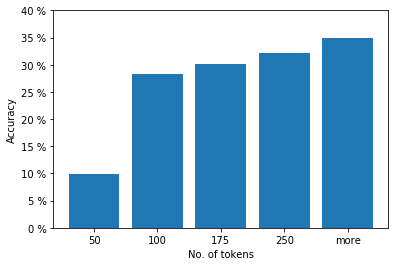
\includegraphics[width=\textwidth]{figures/supervised_approach/sm_hw_length.png}
    \caption{Handwritten subjects}
    \label{fig:sm_hw_length}
  \end{subfigure}
  \begin{subfigure}[t]{.32\textwidth}
    \centering
    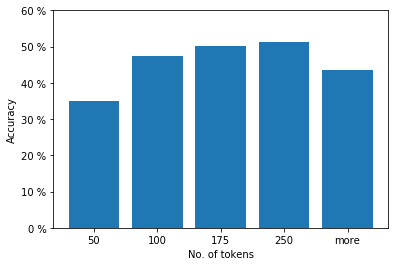
\includegraphics[width=\textwidth]{figures/supervised_approach/sm_ddc_length.png}
    \caption{DDC subjects}
    \label{fig:sm_ddc_length}
  \end{subfigure}
   \begin{subfigure}[t]{.32\textwidth}
    \centering
    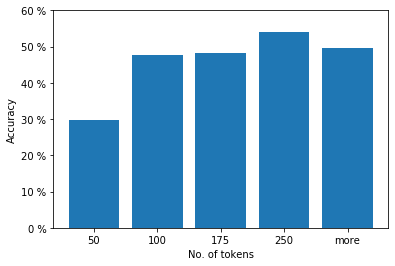
\includegraphics[width=\textwidth]{figures/supervised_approach/sm_venue_length.png}
    \caption{Venues}
    \label{fig:sm_venue_length}
  \end{subfigure}
  \caption{Hit rate of the approaches for the evaluation sets, grouped by representation length. We consider 20 candidates for the handwritten set, and 1 for the two others.}
  \label{fig:sm_eval_length}
\end{figure}

In this section, we analyze how the length of the documents affects the hit rate of the \acrshort{sm}, our most accurate model. We already showed the representation lengths of the documents after mapping their tokens to the pre-trained vectors in figure \ref{fig:sm_doc_length}. Over 8,000 documents were represented by less than 50 word vectors, and over 6,000 documents have less than 100 vectors. Here, we compute the accuracies on the evaluation set for each length group.

Figure \ref{fig:sm_eval_length} shows the accuracies of the \acrshort{sm} on the evaluation sets for the different length groups. In contrast to the other figures displaying model hit rate, here the number of candidates is fixed. Instead of considering all documents at once, we compute the hit rate for each length group. The hit rate for documents with less than 50 tokens is significantly worse than for documents with more than 50 tokens. The difference in the \acrshort{ddc} and venue sets between the shortest documents and the rest ranges between 15 and 20 \% for the most part. For the handwritten set, the difference is even larger: between 20 and 25 \%. This shows that the model's hit rate is considerably hindered when the representation of the document comprises less than 50 vectors.

The hit rate of the model steadily increases with longer representations, but at a much lower rate. Recall that representations with more than 250 tokens are truncated; only the first 250 tokens are fed to the model. We thus conclude that the representation length does impact the hit rate of the model. Documents represented with less than 50 documents are especially challenging for the model. If we discarded these documents, the hit rate of the model would increase by at least 20 \% on all evaluation sets.